%! Author = crist
%! Date = 03/07/2025

\spacing{1.3}


\section{Forces}
\begin{definition}[Force]
        A \textbf{force} is a physical quantity that represents any action capable of modifying the shape of a body or changing the state of rest or motion of that body.
\end{definition}
The unit of force in the International System is the Newton (\unit{\newton}).
We can define one Newton as the force that produces on a body of one kilogram an acceleration of one \unit{\mpss}.

In nature there are four fundamental forces:
\begin{itemize}
    \item Gravitational Force.
    \item Electromagnetic Force.
    \item Strong Nuclear Force.
    \item Weak Nuclear Force.
\end{itemize}

In this chapter we will study the gravitational force and the electromagnetic force, which we will separate into electric force (within the electromagnetic force).

\subsection{Parts of a force: representation of a force}

To correctly represent a force, it is necessary to know that it has four elements:

\begin{itemize}
    \item \textbf{Point of application}.
    The location where the force is applied.
    It is usually indicated with a point, although it is quite common to omit it.
    \item \textbf{Magnitude}.
    Indicates the amount of force being applied, that is, the numerical value.
    \item \textbf{Direction}.
    Indicates where the force is applied (horizontal, vertical or inclined) and is represented by a straight line.
    The greater the magnitude, the longer the line.
    \item \textbf{Sense}.
    Shows to which side the force points and is represented with an arrowhead.
    Numerically, the sense is indicated with a positive or negative sign.
    One direction is always chosen; if the force is positive, it means it is directed towards the chosen direction, while if it is negative, it is directed in the opposite sense.
\end{itemize}

\begin{figure}[H]
    \centering
    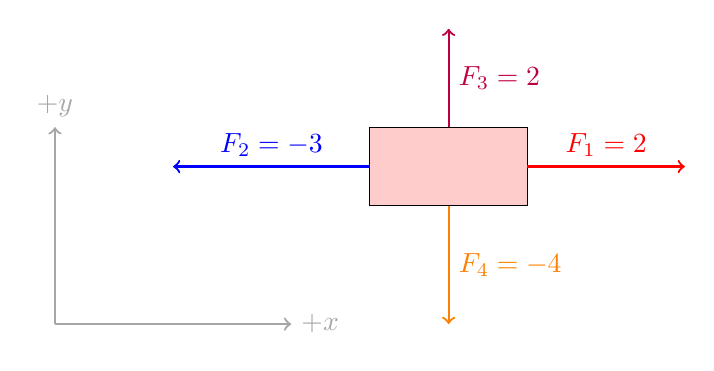
\begin{tikzpicture}

        % Positive axes
        \draw[->, thick, gray!70] (-4,-1.5) -- ++(0,2.5) node[above] {$+y$};
        \draw[->, thick, gray!70] (-4,-1.5) -- ++(3,0) node[right] {$+x$};

        % Block
        \draw[fill=red!20] (0,0) rectangle (2,1);

        % Force F1 (horizontal right)
        \draw[->, thick, red] (2,0.5) -- +(2,0)
        node[midway, above] {$F_1 = \qty{2}{\newton}$};

        % Force F2 (horizontal left)
        \draw[->, thick, blue] (0,0.5) -- +(-2.5,0)
        node[midway, above] {$F_2 = \qty{-3}{\newton}$};

        % Force F3 (vertical upward)
        \draw[->, thick, purple] (1,1) -- +(0,1.25)
        node[midway, right] {$F_3 = \qty{2}{\newton}$};

        % Force F4 (vertical downward)
        \draw[->, thick, orange] (1,0) -- +(0,-1.5)
        node[midway, right] {$F_4 = \qty{-4}{\newton}$};

    \end{tikzpicture}
    \caption{Representation of forces}
    \label{fig:representacion_fuerzas}
\end{figure}

\begin{exercise}
    In your notebook, draw the forces below, applied at the origin of the XY coordinates:
    \begin{enumerate}[label=\letraminuscula]
        \item a force of 5 N, in a horizontal direction to the right.
        \item a force equal to the previous one, but in the
        opposite direction.
        \item a vertical force of 10 N, pointing upwards.
    \end{enumerate}
    \begin{solu}
        Students should draw a coordinate system with the origin at the center, then draw three force vectors:

        \textbf{a)} Draw an arrow pointing to the right along the positive X-axis with magnitude 5 N. Label it as $\vec{F}_1 = 5$ N.

        \textbf{b)} Draw an arrow pointing to the left along the negative X-axis with magnitude 5 N. Label it as $\vec{F}_2 = -5$ N or $\vec{F}_2 = 5$ N to the left.

        \textbf{c)} Draw an arrow pointing upward along the positive Y-axis with magnitude 10 N. Label it as $\vec{F}_3 = 10$ N.

        The arrows should be drawn to scale, so the 10 N force should be twice as long as the 5 N forces. All forces originate from the origin of the coordinate system.
    \end{solu}
\end{exercise}

\subsection{Operations with forces: sum of forces}

In Physics, the symbol \( \Sigma \) indicates that all the present magnitudes must be added.
If we have \( \Sigma F \), it means that we must add all the forces acting on the object.

We can have the following cases:

\begin{itemize}
    \item \textbf{Forces with the same sense}.
    Both will have a positive sign.
    \begin{figure}[H]
        \centering
        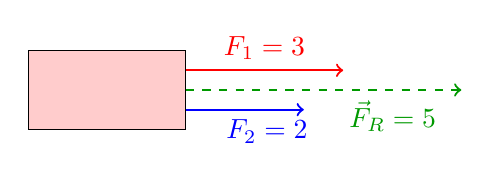
\begin{tikzpicture}
            % Block
            \draw[fill=red!20] (0,0) rectangle (2,1);

            % Force 1 (to the right)
            \draw[->, thick, red] (2,0.75) -- +(2,0) node[midway, above] {$F_1 = \qty{3}{\newton}$};

            % Force 2 (to the right)
            \draw[->, thick, blue] (2,0.25) -- +(1.5,0) node[midway, below,xshift=8] {$F_2 = \qty{2}{\newton}$};

            % Resultant force (to the right)
            \draw[->, thick, dashed, green!60!black] (2,0.5) -- +(3.5,0)
            node[midway, below, xshift=25] {$\vec{F}_R = \qty{5}{\newton}$};
        \end{tikzpicture}
        \caption{Forces with the same sense.}
    \end{figure}
    In this case, the resultant force \( F_R \), that is the sum of \( F_1 \) and \( F_2 \), will be:
    \( \Sigma F_R = F_1 + F_2 = \qty{3}{\newton} + \qty{2}{\newton} = \qty{5}{\newton} \).

    \item \textbf{Forces with opposite sense}.
    Now one of the forces will have a negative sign; in the following example it will be \( F_2 \).
    \begin{figure}[H]
        \centering
        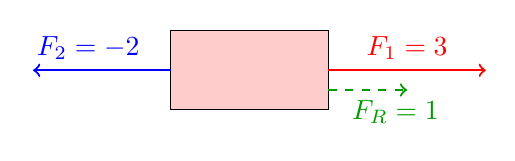
\begin{tikzpicture}
            % Block
            \draw[fill=red!20] (0,0) rectangle (2,1);

            % Force 1 (to the right)
            \draw[->, thick, red] (2,0.5) -- +(2,0) node[midway, above] {$F_1 = \qty{3}{\newton}$};

            % Force 2 (to the left)
            \draw[->, thick, blue] (0,0.5) -- +(-1.75,0) node[midway, above, xshift=-5] {$F_2= \qty{-2}{\newton}$};

            % Resultant force (to the right)
            \draw[->, thick, dashed, green!60!black] (2,0.25) -- +(1,0)
            node[midway, below, xshift=10] {$F_R = \qty{1}{\newton}$};
        \end{tikzpicture}
        \caption{Two forces with opposite sense.}
    \end{figure}
    In this case, we have:
    \( \Sigma F_R = F_1 + F_2 = \qty{3}{\newton} - \qty{2}{\newton} = \qty{1}{\newton} \).
    Since \( F_2 \) goes in the opposite direction, we assign it the negative sign.

    \item \textbf{Two perpendicular forces}.
    To obtain the resultant force, we must apply the Pythagorean theorem.
    \begin{figure}[H]
        \centering
        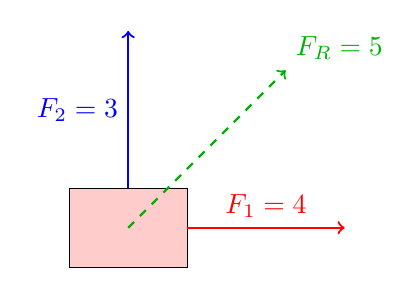
\begin{tikzpicture}
            % Block
            \draw[fill=red!20] (0,0) rectangle (1.5,1);

            % Force F1 (horizontal, right)
            \draw[->, thick, red] (1.5,0.5) -- +(2,0)
            node[midway, above] {$F_1 = \qty{4}{\newton}$};

            % Force F2 (vertical, upward)
            \draw[->, thick, blue] (0.75,1) -- +(0,2)
            node[midway, left] {$F_2 = \qty{3}{\newton}$};

            % Resultant vector
            \draw[->, thick, green!70!black, dashed] (0.75,0.5) -- +(2,2)
            node[above right] {$F_R = \qty{5}{\newton}$};
        \end{tikzpicture}
        \caption{Two perpendicular forces.}
        \label{fig:two_perpendicular_forces}
    \end{figure}
    In this case:
    \( F_R^2 = F_1^2 + F_2^2 \;\;\longrightarrow\;\; F_R = \sqrt{F_1^2 + F_2^2} \).

    \( F_R = \sqrt{3^2 + 4^2} = \qty{5}{\newton} \).
\end{itemize}


\begin{exercise}
    Two horses pull a cart in the same direction with a force of 300 N each.
    Calculate the magnitude and direction of the resultant force.


    \begin{solu}
        Since both horses pull in the same direction, the forces are parallel and in the same sense, so we simply add their magnitudes.

        \textbf{Given data:}
        \begin{itemize}
            \item $F_1 = 300$ N
            \item $F_2 = 300$ N
            \item Both forces in the same direction
        \end{itemize}

        \textbf{Solution:}

        The resultant force is:
        $$F_R = F_1 + F_2 = 300\text{ N} + 300\text{ N} = 600\text{ N}$$

        \textbf{Answer:} The magnitude of the resultant force is 600 N, and its direction is the same as the direction in which both horses are pulling (forward).
    \end{solu}
\end{exercise}



\begin{exercise}
    Draw the forces shown below, applied at the origin of the X- and Y-axes:
    \begin{enumerate}[label=\letraminuscula]
        \item a force of magnitude 6 N, downwards.
        \item a force the same as in a., but in the opposite direction.
        \item a force of magnitude 7 N, horizontal direction and to the left.
        \item a force of magnitude 4 N and whose direction forms an angle of 45° with the positive X-axis.
    \end{enumerate}


    \begin{solu}
        Students should draw a coordinate system with the origin at the center, then draw four force vectors:

        \textbf{a)} Draw an arrow pointing downward along the negative Y-axis with magnitude 6 N. Label it as $\vec{F}_1 = 6$ N downward.

        \textbf{b)} Draw an arrow pointing upward along the positive Y-axis with magnitude 6 N. Label it as $\vec{F}_2 = 6$ N upward.

        \textbf{c)} Draw an arrow pointing to the left along the negative X-axis with magnitude 7 N. Label it as $\vec{F}_3 = 7$ N to the left.

        \textbf{d)} Draw an arrow at a 45° angle from the positive X-axis (pointing into the first quadrant) with magnitude 4 N. This vector should make equal angles with both axes. Label it as $\vec{F}_4 = 4$ N at 45°.

        All vectors should originate from the origin and be drawn to scale.
    \end{solu}
\end{exercise}


\begin{exercise}
    Two colleagues push a table in the same direction with forces of 110 N and 135 N. Find the resultant force with which they push the table.
    Draw the force diagram.


    \begin{solu}
        Since both colleagues push in the same direction, we add the forces algebraically.

        \textbf{Given data:}
        \begin{itemize}
            \item $F_1 = 110$ N
            \item $F_2 = 135$ N
            \item Both forces in the same direction
        \end{itemize}

        \textbf{Solution:}
        $$F_R = F_1 + F_2 = 110\text{ N} + 135\text{ N} = 245\text{ N}$$

        \textbf{Force diagram:} Draw two arrows pointing in the same direction (e.g., to the right) labeled 110 N and 135 N. Then draw a longer arrow in the same direction labeled 245 N representing the resultant force.

        \textbf{Answer:} The resultant force is 245 N in the direction they are both pushing.
    \end{solu}
\end{exercise}


\begin{exercise}
    These two dogs pull on each end of a rubber toy.
    The dog on the right pulls with a force of magnitude 80 N and the one on the left with a force of 95 N.
    \begin{enumerate}[label=\letraminuscula]
        \item Find the magnitude and direction of the resultant force.
        \item Draw a force diagram of the two forces and
        the resultant force.
    \end{enumerate}


    \begin{solu}
        \textbf{a) Magnitude and direction of the resultant force:}

        Since the dogs pull in opposite directions, we subtract the forces. Taking the right direction as positive:

        \textbf{Given data:}
        \begin{itemize}
            \item $F_{right} = 80$ N (to the right)
            \item $F_{left} = 95$ N (to the left)
        \end{itemize}

        $$F_R = F_{right} - F_{left} = 80\text{ N} - 95\text{ N} = -15\text{ N}$$

        The negative sign indicates the direction is to the left.

        \textbf{Answer:} The magnitude of the resultant force is 15 N, directed to the left (in the direction of the dog pulling with more force).

        \textbf{b) Force diagram:} Draw two arrows pointing in opposite directions: one to the right labeled 80 N and one to the left labeled 95 N. Then draw a shorter arrow to the left labeled 15 N representing the resultant force.
    \end{solu}
\end{exercise}




\begin{exercise}
    The result of two perpendicular forces applied to a body is 25 N.
    If one of the forces has a magnitude of 7 N, find the magnitude of the other force.


    \begin{solu}
        We use the Pythagorean theorem since the forces are perpendicular.

        \textbf{Given data:}
        \begin{itemize}
            \item $F_R = 25$ N (resultant force)
            \item $F_1 = 7$ N (one of the forces)
            \item $F_2 = ?$ (unknown force)
            \item Forces are perpendicular
        \end{itemize}

        \textbf{Solution:}

        From the Pythagorean theorem:
        $$F_R^2 = F_1^2 + F_2^2$$

        Solving for $F_2$:
        $$F_2 = \sqrt{F_R^2 - F_1^2} = \sqrt{(25)^2 - (7)^2} = \sqrt{625 - 49} = \sqrt{576} = 24\text{ N}$$

        \textbf{Answer:} The magnitude of the other force is 24 N.
    \end{solu}
\end{exercise}



\begin{exercise}
    Two groups of students pull on an object, with the same force of 250 N, using ropes attached to opposite sides of the object.
    \begin{enumerate}[label=\letraminuscula]
        \item What's the resultant force?
        \item If the group on the right now pulls with a force of 325 N, calculate the resultant force and direction.
    \end{enumerate}

    \begin{solu}
        \textbf{a) Resultant force when both groups pull with 250 N:}

        Since the groups pull in opposite directions with equal magnitude, the forces cancel each other out.

        Taking the right direction as positive:
        $$F_R = F_{right} - F_{left} = 250\text{ N} - 250\text{ N} = 0\text{ N}$$

        \textbf{Answer:} The resultant force is 0 N. The object remains in equilibrium.

        \textbf{b) Resultant force when the right group pulls with 325 N:}

        Now the forces are unequal:
        $$F_R = F_{right} - F_{left} = 325\text{ N} - 250\text{ N} = 75\text{ N}$$

        \textbf{Answer:} The resultant force is 75 N directed to the right (in the direction of the stronger force).
    \end{solu}
\end{exercise}





\begin{exercise}
    Two separate forces, each of 100 N, act on the same object at an angle of \ang{90}.
    Find the magnitude of the resultant force and draw its direction on a force diagram.

    \begin{solu}
        When two forces are perpendicular to each other, we use the Pythagorean theorem to find the magnitude of the resultant force.

        \textbf{Given data:}
        \begin{itemize}
            \item $F_1 = 100$ N
            \item $F_2 = 100$ N
            \item Angle between forces = 90°
        \end{itemize}

        \textbf{Solution:}

        Using the Pythagorean theorem:
        $$F_R = \sqrt{F_1^2 + F_2^2} = \sqrt{(100)^2 + (100)^2} = \sqrt{10000 + 10000} = \sqrt{20000} = 141.42\text{ N}$$

        The direction of the resultant force forms an angle of 45° with each of the original forces (since they are equal and perpendicular).

        \textbf{Force diagram:} Draw two perpendicular arrows of equal length (100 N each), one horizontal and one vertical. Then draw the resultant as the diagonal of the rectangle formed, labeled 141.42 N, at 45° from each original force.

        \textbf{Answer:} The magnitude of the resultant force is approximately 141.42 N, directed at 45° from each original force.
    \end{solu}
\end{exercise}


\section{Deformation of Bodies}


We have previously seen that a force can produce a deformation.
We can mainly distinguish two types of deformation:

\begin{itemize}
    \item \textbf{Plastic Deformation}: occurs when the deformed body does not recover its original shape after the force ceases.
    It is an irreversible and permanent process.
    \item \textbf{Elastic Deformation}: is the deformation that disappears when the external force that produced it stops.
    In this unit, we will study this type of deformation.
\end{itemize}

\subsection{Elastic Force: Hooke's Law}

This type of force refers to the forces that arise when we deform an elastic material.

Thus, under the action of a force, a spring may experience elongation or compression until the force disappears.

\begin{dBox}
    \textbf{Hooke's Law}: the deformation of an elastic spring is proportional to the deforming force.
    The elastic force we calculate in a given spring will be equal in magnitude and direction but opposite in sense to the force causing that deformation (later we will see that this corresponds to Newton's 3rd law).
\end{dBox}

\begin{remark}
    The elastic force will always have a negative sign because it opposes the direction of the applied force.
    We will not include the sign here because we are only determining the magnitude, not the direction.
\end{remark}

\vspace*{20pt}
\begin{centeredequation}
    \eqnmarkbox[blue]{elasticforce}{F_{\text{elastic}}}
    =
    \eqnmarkbox[red]{springconstant}{k}
    \cdot
    \eqnmarkbox[mygreen]{elongation}{\Delta l}
\end{centeredequation}
\annotate[yshift=1em]{left}{elasticforce}{Elastic force}
\annotate[yshift=1em]{}{springconstant}{Spring constant specific to each spring}
\annotate[yshift=-2em]{below,left}{elongation}{Length by which the spring has been stretched or compressed}
\vspace*{12pt}

To calculate \( \Delta l \), we can use the expression: \( \Delta l = l_f - l_i \), where \( l_f \) is the final length of the spring and \( l_i \) is the initial length of the spring.

\begin{remark}
    If we are told that a spring has stretched or compressed by a certain distance, this directly gives us the value of \( \Delta l \).
\end{remark}

Each spring has its own spring constant, with units in the International System of \unit{\newton\per\metre}.

\subsection{Measurement of Forces}

\begin{minipage}{0.6\textwidth}
    To measure forces, a \textbf{dynamometer} is used.

    A dynamometer is an instrument with a spring that has a known spring constant.
    This spring has an attached scale calibrated in newtons, which allows us to measure forces.
    To calculate these forces, we use Hooke's law studied previously.

    Its use is basic: if we want to calculate the force exerted by an object (usually its weight), we hang the object from the hook of the dynamometer.
\end{minipage}
\hfill
\begin{minipage}{0.35\textwidth}
    \begin{figure}[H]
        \centering
%        \includegraphics[scale=0.20]{images/dinamica/dinanometro}
        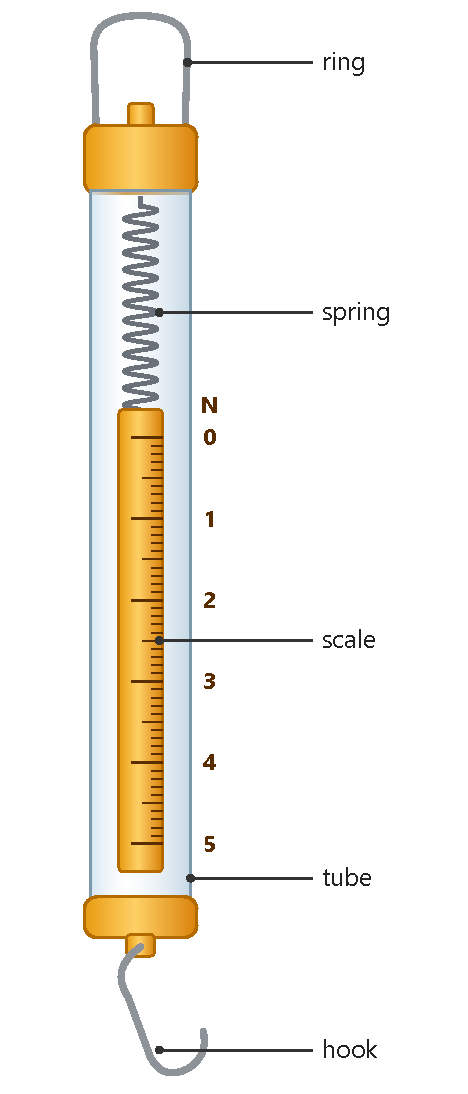
\includegraphics[width=0.6\linewidth]{Figuras_SVG_ENG/pdf/U3_dinamometro.pdf}
        \caption{Dynamometer}
        \label{fig:dinamometro}
    \end{figure}
    \vspace{6pt}
\end{minipage}

We said previously that the force exerted by an object is equal to the elastic force, so we can apply:
\begin{centeredequation}
    F_{\text{elastic}} = F_{\text{object}}
\end{centeredequation}

Since we know the spring constant of the dynamometer and measure the elongation of the spring, we can easily calculate the object's force using:
\begin{centeredequation}
    F_{\text{object}} = k \cdot \Delta l
\end{centeredequation}

\begin{exercise}
    When a force of 20 N is applied to a certain spring, it produces an elongation of 10 cm.
    \begin{enumerate}[label=\alph*)]
        \item Calculate the spring constant.
        \item Calculate the elongation of the spring when a force of 200 N is applied.
        \item Determine the force required to produce an elongation of 5 dm.
    \end{enumerate}

    \begin{solu}
        We use Hooke's Law: $F = k \cdot \Delta x$

        \textbf{Given data:}
        \begin{itemize}
            \item $F = 20$ N
            \item $\Delta x = 10$ cm = 0.10 m
        \end{itemize}

        \textbf{a) Calculate the spring constant:}

        From Hooke's Law:
        $$k = \frac{F}{\Delta x} = \frac{20\text{ N}}{0.10\text{ m}} = 200\text{ N/m}$$

        \textbf{Answer:} The spring constant is 200 N/m.

        \textbf{b) Elongation when F = 200 N:}

        $$\Delta x = \frac{F}{k} = \frac{200\text{ N}}{200\text{ N/m}} = 1\text{ m} = 100\text{ cm}$$

        \textbf{Answer:} The elongation is 1 m or 100 cm.

        \textbf{c) Force required for an elongation of 5 dm:}

        First, convert: 5 dm = 0.5 m

        $$F = k \cdot \Delta x = 200\text{ N/m} \times 0.5\text{ m} = 100\text{ N}$$

        \textbf{Answer:} A force of 100 N is required.
    \end{solu}
\end{exercise}

\begin{exercise}
    In an experiment to determine the spring constant, the following results were obtained:
    \begin{table}[H]
        \centering
        \renewcommand{\arraystretch}{1.5}
        \begin{tabular}{Occccc}
            \bottomrule
            \textcolor{ocre}{\textbf{F (\unit{\newton})}}      & 0 & 5   & 10 & 15 & 20  \\
            \hline
            \textcolor{ocre}{\textbf{x (\unit{\centi\metre})}} & 0 & 2.1 & 4  & 6  & 7.9 \\
            \toprule
        \end{tabular}
        \label{tab:ejercicio1}
    \end{table}
%    \begin{figure}[H]
%        \centering
%        \includegraphics{images/dinamica/ejercicio_9}
%    \end{figure}
    \begin{enumerate}[label=\alph*)]
        \item Plot the data from the table on a graph.
        \item What is the value of the spring constant?
    \end{enumerate}

    \begin{solu}
        \textbf{Note:} Since the image with the data table is not available in the text, I'll provide a general solution method.

        \textbf{a) Plotting the data:}

        Students should create a graph with:
        \begin{itemize}
            \item X-axis: Extension/Elongation ($\Delta x$) in meters
            \item Y-axis: Force (F) in Newtons
            \item Plot all the data points from the table
            \item Draw a best-fit straight line through the origin
        \end{itemize}

        \textbf{b) Calculating the spring constant:}

        According to Hooke's Law: $F = k \cdot \Delta x$

        This is a linear relationship of the form $y = mx$ where:
        \begin{itemize}
            \item The slope ($m$) equals the spring constant ($k$)
            \item $k = \frac{F}{\Delta x}$ or $k = \frac{\Delta F}{\Delta \Delta x}$
        \end{itemize}

        To find $k$:
        \begin{enumerate}
            \item Choose two points from the line: $(x_1, y_1)$ and $(x_2, y_2)$
            \item Calculate the slope: $k = \frac{y_2 - y_1}{x_2 - x_1} = \frac{F_2 - F_1}{\Delta x_2 - \Delta x_1}$
        \end{enumerate}

        \textbf{Answer:} The spring constant is the slope of the Force vs. Extension graph, measured in N/m.
    \end{solu}
\end{exercise}

\begin{exercise}
    Find the force required to stretch a spring with a constant of 150 N/m by 3 cm from its initial length.

    \begin{solu}
        We use Hooke's Law: $F = k \cdot \Delta x$

        \textbf{Given data:}
        \begin{itemize}
            \item $k = 150$ N/m
            \item $\Delta x = 3$ cm = 0.03 m
        \end{itemize}

        \textbf{Solution:}
        $$F = k \cdot \Delta x = 150\text{ N/m} \times 0.03\text{ m} = 4.5\text{ N}$$

        \textbf{Answer:} A force of 4.5 N is required to stretch the spring by 3 cm.
    \end{solu}
\end{exercise}


\section{Newton's Laws}

\subsection{First Law of Newton: Law of Inertia}

Known as the \textbf{Law of Inertia}, it states the following:
\begin{dBox}
    \textbf{First Law of Newton: Law of Inertia}. Every body remains at rest or in uniform straight-line motion unless acted upon by an external force.
\end{dBox}

\subsection{Second Law of Newton: Fundamental Principle of Dynamics}

\begin{dBox}
    \textbf{Second Law of Newton: Fundamental Principle of Dynamics}. The acceleration of a body is directly proportional to the force applied to that body. Moreover, the change in velocity of the body occurs along the line of action of the applied force.
    \begin{centeredequation}
        \Sigma F = m\ a
    \end{centeredequation}
\end{dBox}

\begin{exercise}
    A force of 5 N is applied to a body of mass 0.2 kg.
    What acceleration will the body acquire?

    \begin{solu}
        We use Newton's Second Law: $F = m \cdot a$
        \textbf{Given data:}
        \begin{itemize}
            \item $F = 5$ N
            \item $m = 0.2$ kg
        \end{itemize}

        \textbf{Solution:}

        Solving for acceleration:
        $$a = \frac{F}{m} = \frac{5\text{ N}}{0.2\text{ kg}} = 25\text{ m/s}^2$$

        \textbf{Answer:} The body will acquire an acceleration of 25 m/s².
    \end{solu}
\end{exercise}

\begin{exercise}
    A man with a mass of 75 kg is sitting in a car that starts moving with an acceleration of 1.5 m/s².
    What force does the man experience?

    \begin{solu}
        We use Newton's Second Law: $F = m \cdot a$

        \textbf{Given data:}
        \begin{itemize}
            \item $m = 75$ kg
            \item $a = 1.5$ m/s²
        \end{itemize}

        \textbf{Solution:}
        $$F = m \cdot a = 75\text{ kg} \times 1.5\text{ m/s}^2 = 112.5\text{ N}$$

        \textbf{Answer:} The man experiences a force of 112.5 N in the direction of the car's acceleration. This force is exerted by the seat pushing him forward.
    \end{solu}
\end{exercise}

\begin{exercise}
    Calculate the horizontal force being applied to a body of mass 25 kg moving at a constant velocity of 25 km/h on a horizontal surface.

    \begin{solu}
        According to Newton's First Law, if a body moves at constant velocity, the net force acting on it is zero.

        \textbf{Given data:}
        \begin{itemize}
            \item $m = 25$ kg
            \item $v = 25$ km/h = constant
        \end{itemize}

        \textbf{Solution:}

        If the velocity is constant, the acceleration is zero:
        $$a = 0\text{ m/s}^2$$

        Using Newton's Second Law:
        $$F_{net} = m \cdot a = 25\text{ kg} \times 0\text{ m/s}^2 = 0\text{ N}$$

        This means that if there is friction, the applied horizontal force must equal the friction force to maintain constant velocity. However, if we assume no friction (or the question asks for the net force), the answer is 0 N.

        \textbf{Answer:} The net horizontal force is 0 N, since the body moves at constant velocity (no acceleration). If there is friction, the applied force equals the friction force, but the net force is still zero.
    \end{solu}
\end{exercise}

\begin{exercise}
    Calculate the force that a person must apply to a table of mass 20 kg to give it an acceleration of \qty{1.25}{\mpss}.
    If someone is on the opposite side of the table, what force must be applied to prevent it from moving?

    \begin{solu}
        We use Newton's Second Law: $F = m \cdot a$

        \textbf{Given data:}
        \begin{itemize}
            \item $m = 20$ kg
            \item $a = 1.25$ m/s²
        \end{itemize}

        \textbf{Solution for the first part:}
        $$F = m \cdot a = 20\text{ kg} \times 1.25\text{ m/s}^2 = 25\text{ N}$$

        \textbf{Answer:} The person must apply a force of 25 N.

        \textbf{Solution for the second part:}

        To prevent the table from moving, the person on the opposite side must apply an equal force in the opposite direction to create equilibrium (net force = 0).

        \textbf{Answer:} The person on the opposite side must apply a force of 25 N in the opposite direction to prevent the table from moving.
    \end{solu}
\end{exercise}

\begin{exercise}
    Two girls are pushing a 50 kg wooden cabinet across a horizontal floor.
    Each of them exerts a force of 25 N. Find the cabinet's acceleration.
    What is its direction relative to the girls?

    \begin{solu}
        We use Newton's Second Law: $F = m \cdot a$

        \textbf{Given data:}
        \begin{itemize}
            \item $m = 50$ kg
            \item $F_1 = 25$ N
            \item $F_2 = 25$ N
            \item Assuming both girls push in the same direction
        \end{itemize}

        \textbf{Solution:}

        First, calculate the total force:
        $$F_{total} = F_1 + F_2 = 25\text{ N} + 25\text{ N} = 50\text{ N}$$

        Then, apply Newton's Second Law:
        $$a = \frac{F_{total}}{m} = \frac{50\text{ N}}{50\text{ kg}} = 1\text{ m/s}^2$$

        \textbf{Answer:} The cabinet's acceleration is 1 m/s². The direction is the same as the direction in which both girls are pushing (assuming they push in the same direction).
    \end{solu}
\end{exercise}

\subsection{Third Law of Newton: Action and Reaction Law}

\begin{dBox}
    \textbf{Third Law of Newton: Action and Reaction Law}: When two bodies interact, they exert forces on each other that are equal in magnitude but opposite in direction.
\end{dBox}

If we denote the force that object A exerts on object B as (\( F_{AB} \)) and the force that object B exerts on object A as (\( F_{BA} \)), we have:
\begin{centeredequation}
    F_{AB} = - F_{BA}
\end{centeredequation}


\section{Gravitational Force}

It is one of the four fundamental forces and is responsible for the structure of the universe.
It is an interaction that occurs between two bodies with mass, is \textbf{always attractive}, and has unlimited range.

In the 17th century, Isaac Newton considered that the force the Earth exerts on the Moon is the same as that exerted on any body on the Earth's surface — gravitational attraction.
He extended this interaction to all planets, stating that gravity is an attribute of all bodies and is proportional to the amount of matter contained in each.

The intensity of the gravitational force depends on the masses of the bodies and the distance between them.
Thus, the greater the mass of a body, the greater the gravitational force it produces.
However, the greater the distance between the bodies, the smaller the gravitational force.
Gravitational force is usually represented by \( F_G \) and is expressed as:

\begin{centeredequation}
    F_G = G \cdot \dfrac{m_1 \cdot m_2}{r^2}
\end{centeredequation}

Where \( G \) is the universal gravitational constant with a value of \( G = \qty{6.67e-11}{\newton\square\metre\per\square\kilo\g} \), \( m_1 \) and \( m_2 \) are the masses of the two bodies, and \( r \) is the distance between them.
Since gravitational force is a force, it is measured in Newtons.

\begin{remark}
    The distance between the two objects is always measured from the centre of each object.
\end{remark}

\begin{remark}
    For planets, measure the distance from the centre of each planet, and because they are large, you must know the radius of each planet.
\end{remark}

If we want to calculate the gravitational force that the Earth exerts on an object on its surface with mass \( m \), we apply the following equation:
\vspace*{31pt}
\begin{centeredequation}
    \eqnmarkbox[red]{gravitationalforce}{F_G}
    =
    G \cdot
    \dfrac{\eqnmarkbox[blue]{earthmass}{M_T} \cdot m}{\eqnmarkbox[mygreen]{earthradius}{R_T^2}}
\end{centeredequation}

\annotate[yshift=1em]{left}{gravitationalforce}{Force exerted by the Earth on the object}
\annotate[yshift=1em]{}{earthmass}{Mass of the Earth}
\annotate[yshift=-2em]{below,left}{earthradius}{Radius of the Earth}
\vspace*{31pt}

If we want to calculate the force that the Earth exerts on an object at a height \( h \) above the Earth's surface, we must add that height \( h \) to the Earth's radius, giving:
\begin{centeredequation}
    F_G = G \cdot \dfrac{M_T \cdot m}{(R_T + h)^2}
\end{centeredequation}

\begin{remark}
    Remember to convert all quantities to SI units before using them in formulas.
\end{remark}

\subsection{Gravity or Gravitational Field}
\begin{definition}[Gravity or Gravitational Field]
Is the attraction generated in space by a mass around it.
\end{definition}

For example, the Earth has a gravitational field on its surface of \qty{9.8}{\mpss}, but this value decreases as we move upward.
As we can see, gravity has the same units as acceleration,\unit{\mpss}
The expression for gravity is:

\begin{centeredequation}
    g = G \cdot \dfrac{m}{r^2}
\end{centeredequation}

Where \( m \) is the mass of the body exerting the gravitational force and \( r \) is the distance between the centre of that body and the point where we want to calculate the gravity.

The formula to calculate gravity at the Earth's surface is:

\begin{centeredequation}
    g_T = G \cdot \dfrac{M_T}{R_T^2}
\end{centeredequation}

To calculate gravity at a height \( h \) above the Earth's surface, the expression is:

\begin{centeredequation}
    g_T = G \cdot \dfrac{M_T}{(R_T+h)^2}
\end{centeredequation}

\begin{remark}
    Gravity on the surface of planets is different, so to calculate it, we must know the mass and radius of the planet.
\end{remark}

\newpage

\begin{centeredequation}
    g_{\text{Planet}} = G \cdot \dfrac{M_{\text{Planet}}}{R_{\text{Planet}}^2}
\end{centeredequation}

\begin{remark}
    Remember to convert all quantities to SI units before using them in formulas.
\end{remark}

\subsection{Weight Force (p or w)}

In fact, the gravitational force is called \textbf{Weight}.

\begin{definition}[Weight Force]
    Is the force with which the Earth, or any other planet, attracts the bodies on it.
    Given the mass of any person or object on the Earth or another planet, the weight of that object or person is given by:
    \begin{centeredequation}
        w = m \cdot g \quad \text{or} \quad p = m \cdot g
    \end{centeredequation}
    Where \( m \) is the mass of the object and \( g \) is the gravity of that planet.
\end{definition}

Since weight is a force, its unit is Newton.

As we can see from the weight formula, this force depends on the mass of each object as well as the gravity of the planet we are on.

\begin{remark}
    Gravity on the Moon is different from that on Earth; therefore, to calculate weight on the Moon, we must first calculate the gravity on the Moon.
\end{remark}

\begin{exercise}
    European Space Agency Meteosat satellites have a mass of 2000 kg and orbit the Earth in a circular path at a radius of 36000 km.
    Calculate the force with which the Earth attracts these satellites.
    What is the effect of this force on the satellites?

    \datos{} \Ggravitacion; \( M_T = \qty{5.99e24}{\kilo\g} \); \( R_T = \qty{6380}{\kilo\metre} \)

    \begin{solu}
        We use Newton's Law of Universal Gravitation: $F = \frac{G \cdot M_1 \cdot M_2}{r^2}$

        \textbf{Given data:}
        \begin{itemize}
            \item $G = 6.67 \times 10^{-11}$ N·m²/kg²
            \item $M_{Earth} = 5.99 \times 10^{24}$ kg
            \item $m_{satellite} = 2000$ kg
            \item $r = 36000$ km = $3.6 \times 10^7$ m (orbital radius from Earth's center)
        \end{itemize}

        \textbf{Solution}
    \end{solu}
\end{exercise}



\begin{exercise}
    On a certain planet, we measure the weight of a 9 kg mass with a dynamometer and obtain a reading of 108 N. What is the value of \( g \) on that planet?
    \begin{solu}
        We use the relationship between weight and mass: $W = m \cdot g$

        \textbf{Given data:}
        \begin{itemize}
            \item $m = 9$ kg
            \item $W = 108$ N
        \end{itemize}

        \textbf{Solution:}

        Solving for $g$:
        $$g = \frac{W}{m} = \frac{108\text{ N}}{9\text{ kg}} = 12\text{ m/s}^2$$

        \textbf{Answer:} The value of $g$ on that planet is 12 m/s².
    \end{solu}
\end{exercise}

\begin{exercise}
    From astronomical observations, we know that Jupiter has a radius of \qty{6.98e7}{\metre} and a mass of \qty{1.9e27}{\kilo\g}.
    Calculate the acceleration due to gravity on this planet.

    \datos{}: \Ggravitacion

    \begin{solu}
        We use the formula for gravitational acceleration: $g = \frac{G \cdot M}{R^2}$

        \textbf{Given data:}
        \begin{itemize}
            \item $G = 6.67 \times 10^{-11}$ N·m²/kg²
            \item $M_{Jupiter} = 1.9 \times 10^{27}$ kg
            \item $R_{Jupiter} = 6.98 \times 10^{7}$ m
        \end{itemize}

        \textbf{Solution:}
        $$g_{Jupiter} = \frac{G \cdot M_{Jupiter}}{R_{Jupiter}^2} = \frac{6.67 \times 10^{-11} \times 1.9 \times 10^{27}}{(6.98 \times 10^7)^2}$$

        $$g_{Jupiter} = \frac{1.267 \times 10^{17}}{4.872 \times 10^{15}} = 26.0\text{ m/s}^2$$

        \textbf{Answer:} The acceleration due to gravity on Jupiter is approximately 26.0 m/s², which is about 2.65 times stronger than Earth's gravity.
    \end{solu}
\end{exercise}



\begin{exercise}
    We hang a 500 g mass on a dynamometer, and its scale reads 4.85 N. What is the value of \( g \)?
\end{exercise}

\begin{exercise}
    We measure the mass of an object using a laboratory scale and find it is 0.9 kg.
    Work with a classmate to calculate its weight.
\end{exercise}


\begin{exercise}
    A boy weighs 441 N on Earth.
    In your notebook, answer the following questions:
    \begin{enumerate}[label=\alph*)]
\item What is the boy’s weight on Mars?
\item What is his mass on the Moon?
\item What is his weight on the Moon?
    \end{enumerate}

    \datos{}: \( g_{\text{Mars}} = \qty{3.7}{\mpss} \); \( g_{\text{Moon}} = \qty{1.6}{\mpss} \)
\end{exercise}


\begin{exercise}
    Mount Chimborazo is the furthest point from the Earth’s centre of gravity, at 6268 m above sea level (which is 6 378 000 metres from the Earth’s centre of mass).
    Find \( g \) on Chimborazo’s summit and compare it to \( g \) at sea level (\qty{9.8}{\mpss}).
\end{exercise}

\begin{exercise}
    The Hubble is a telescope that remains in orbit around the Earth at an altitude of 600 km above its surface.
    Determine the gravitational acceleration the Hubble is subjected to.

    \datos{}: \Ggravitacion; \( M_T = \qty{5.99e24}{\kilo\g} \); \( R_T = \qty{6380}{\kilo\metre} \)
\end{exercise}


\begin{exercise}
    Calculate the weight for a person of 80 kg located at the height of Mount Everest (8848 m).
    And at an altitude of 300 km?

    \datos{}: \Ggravitacion; \( M_T = \qty{5.99e24}{\kilo\g} \); \( R_T = \qty{6380}{\kilo\metre} \)
\end{exercise}


\begin{exercise}
    Calculate the gravity on the Moon. What force does the Moon exert on an astronaut with a mass of 95 kg?

    \datos{}: \Ggravitacion; \( M_L = \qty{7.36e22}{\kilo\g} \); \( R_L = \qty{1740}{\kilo\metre} \)
\end{exercise}


\section{Electric Force}

As we studied previously, the atom is composed of two charged particles: electrons, with negative charge, and protons, with positive electric charge.
Normally, materials have the same number of electrons as protons and are neutral; however, due to \textbf{electrification} processes, there can be a transfer of electrons from one body to another, creating an imbalance between positive and negative charges in a body.

In this type of force, electric charges are involved, and therefore we must define a new quantity that allows us to quantify the value of that charge (equivalent to mass in gravitational force).
\begin{definition}[Electric Charge]
    Is a property of matter present in subatomic particles.
    The unit of electric charge is the Coulomb, represented as \( \unit{\coulomb} \).

    Electric charges can be positive or negative.
\end{definition}

Electric force is another of the four fundamental forces of nature and becomes clear when we have electric charges.
Electric forces can be \textbf{attractive} when charges are of the opposite sign, and \textbf{repulsive} when charges are of the same sign.

In the 18th century, Charles Coulomb discovered the properties of this force and the relationships between charges and their distances, leading to the expression:
\vspace{36pt}

\begin{centeredequation}
    \eqnmarkbox[red]{electricforce}{F_e} =
    \eqnmarkbox[mygreen]{coulombconstant}{K} \cdot
    \dfrac{\eqnmarkbox[blue]{charge1}{q_1} \cdot \eqnmarkbox[blue]{charge2}{q_2}}{\eqnmarkbox[myOrange]{chargedistance}{r^2}}
\end{centeredequation}

\annotate[yshift=1em]{left}{electricforce}{Electric force}
\annotate[yshift=1.25em]{}{coulombconstant}{Coulomb constant}
\annotate[yshift=-2em]{below,left}{charge1}{Charge of particle 1}
\annotate[yshift=-4em]{below,left}{charge2}{Charge of particle 2}
\annotate[yshift=-0.5em,xshift=1.5em]{below}{chargedistance}{Distance between charges}
\vspace{36pt}

\begin{remark}
    For calculations, use the absolute value of the charge, i.e.\ without the sign.
\end{remark}

The Coulomb constant (\( K \)) has a value of \( K = \qty{9e9}{\newton\square\metre\per\square\coulomb} \).

\begin{remark}
    It is crucial to avoid errors to convert all quantities to SI units before substituting them into the formula.
\end{remark}


\begin{exercise}
    Calculate the force between two charges:
    \begin{enumerate}[label=\alph*)]
\item \qty{+5}{\micro\coulomb} and \qty{+3}{\micro\coulomb} located 10 cm apart.
\item \qty{+5}{\micro\coulomb} and \qty{-3}{\micro\coulomb} located 10 cm apart.
    \end{enumerate}

    \datos{}: \ctecoulomb

\end{exercise}


\begin{exercise}
    What is the magnitude of the electric force exerted on a charge of +7 C by another charge of +3 C located 2 m away?
    Is the force attractive or repulsive?

    \datos{}: \ctecoulomb

\end{exercise}

\begin{exercise}
    The mass of a proton is \qty{1.67e-27}{\kilo\g} and its electric charge is \qty{1.6e-19}{\coulomb}.
    Compare the electric repulsion force between two protons in a vacuum at a distance of 1 m with the gravitational attraction between them.

    \datos{}: \ctecoulomb; \Ggravitacion

\end{exercise}


\begin{exercise}
    Make a conceptual map of the unit.
    \begin{solu}
        This is a creative exercise where students should organise the main concepts of the unit in a hierarchical or connected way. The conceptual map should include:

        \textbf{Main concepts to include:}
        \begin{itemize}
            \item Forces: definition, representation (magnitude, direction, point of application)
            \item Types of forces: contact forces (friction, normal, tension) and forces at a distance (gravitational, electric)
            \item Vector addition of forces
            \item Newton's Laws of Motion (First, Second, and Third Law)
            \item Hooke's Law and elastic forces
            \item Weight and mass difference
            \item Universal Law of Gravitation
            \item Coulomb's Law
        \end{itemize}
        Students should create connections between these concepts showing how they relate to each other.
    \end{solu}
\end{exercise}


\section{Vocabulary}

\begin{vocabulary}[Force]
A physical quantity that represents an interaction capable of changing the motion, speed, direction, or shape of an object. \newline
\textbf{Translation to Spanish}: Fuerza \newline
% Line 8
\end{vocabulary}

\begin{vocabulary}[Newton]
The SI unit of force, defined as the force required to accelerate a mass of one kilogram at one meter per second squared. \newline
\textbf{Translation to Spanish}: Newton \newline
% Line 11
\end{vocabulary}

\begin{vocabulary}[Acceleration]
The rate at which the velocity of an object changes with time. \newline
\textbf{Translation to Spanish}: Aceleración \newline
% Line 12
\end{vocabulary}

\begin{vocabulary}[Gravitational Force]
The attractive force that exists between any two masses in the universe. \newline
\textbf{Translation to Spanish}: Fuerza gravitatoria \newline
% Line 16
\end{vocabulary}

\begin{vocabulary}[Electromagnetic Force]
A fundamental force responsible for interactions between electrically charged particles. \newline
\textbf{Translation to Spanish}: Fuerza electromagnética \newline
% Line 17
\end{vocabulary}

\begin{vocabulary}[Strong Nuclear Force]
The fundamental force that holds protons and neutrons together inside the nucleus of an atom. \newline
\textbf{Translation to Spanish}: Fuerza nuclear fuerte \newline
% Line 18
\end{vocabulary}

\begin{vocabulary}[Weak Nuclear Force]
A fundamental force involved in radioactive decay and certain particle interactions. \newline
\textbf{Translation to Spanish}: Fuerza nuclear débil \newline
% Line 19
\end{vocabulary}

\begin{vocabulary}[Vector]
A physical quantity that has both magnitude and direction. \newline
\textbf{Translation to Spanish}: Vector \newline
% Line 84
\end{vocabulary}

\begin{vocabulary}[Equilibrium]
The state in which the net force acting on an object is zero, resulting in no acceleration. \newline
\textbf{Translation to Spanish}: Equilibrio \newline
% Line 337
\end{vocabulary}

\begin{vocabulary}[Weight]
The gravitational force exerted on an object due to the presence of a massive body such as Earth. \newline
\textbf{Translation to Spanish}: Peso \newline
% Line 443
\end{vocabulary}

\begin{vocabulary}[Tension]
A pulling force transmitted through a rope, cable, or string when it is stretched. \newline
\textbf{Translation to Spanish}: Tensión \newline
% Line 536
\end{vocabulary}

\begin{vocabulary}[Inertia]
The tendency of an object to resist changes in its state of motion. \newline
\textbf{Translation to Spanish}: Inercia \newline
% Line 584
\end{vocabulary}

\begin{vocabulary}[Velocity]
A vector quantity that describes the speed of an object together with its direction of motion. \newline
\textbf{Translation to Spanish}: Velocidad \newline
% Line 594
\end{vocabulary}

\begin{vocabulary}[Mass]
A measure of the amount of matter contained in an object. \newline
\textbf{Translation to Spanish}: Masa \newline
% Line 601
\end{vocabulary}

\begin{vocabulary}[Newton's Second Law]
A law stating that the acceleration of an object is proportional to the net force acting on it and inversely proportional to its mass. \newline
\textbf{Translation to Spanish}: Segunda ley de Newton \newline
% Line 605
\end{vocabulary}

\begin{vocabulary}[Net Force]
The overall force acting on an object after all individual forces are combined vectorially. \newline
\textbf{Translation to Spanish}: Fuerza neta \newline
% Line 645
\end{vocabulary}

\begin{vocabulary}[Friction]
A force that opposes the relative motion between two surfaces in contact. \newline
\textbf{Translation to Spanish}: Fricción \newline
% Line 661
\end{vocabulary}

\begin{vocabulary}[Gravity]
The natural phenomenon by which masses attract each other. \newline
\textbf{Translation to Spanish}: Gravedad \newline
% Line 739
\end{vocabulary}

\begin{vocabulary}[Weight Force]
The force exerted on an object due to gravity, usually directed toward the center of the Earth. \newline
\textbf{Translation to Spanish}: Fuerza peso \newline
% Line 827
\end{vocabulary}

\begin{vocabulary}[Electric Charge]
A physical property of matter that causes it to experience a force in an electromagnetic field. \newline
\textbf{Translation to Spanish}: Carga eléctrica \newline
% Line 972
\end{vocabulary}
